\documentclass[tikz,border=10pt]{standalone}
\usetikzlibrary{positioning}
\usepackage{tkz-graph}
\usepackage{rotating}

\usetikzlibrary{arrows}
\usetikzlibrary{arrows.meta}
\tikzset{main node/.style={circle,fill=blue!20,draw,minimum size=1cm,inner sep=0pt}}
\tikzset{simple node/.style={circle, fill=black,draw, inner sep=0pt,minimum size=5pt}}

%https://tex.stackexchange.com/questions/159127/drawing-simple-graph-pattern-with-tikz

\begin{document}

%%%%%%%%%%%%%%%%%%%%%%%%%%%%%%%%%%%%%%%%%%%%%%%%%%%%%%%%%%%%%%%%%%%%%%%%%%%%%%%%%%%%%%%%%%%%%%%%%%%%%%

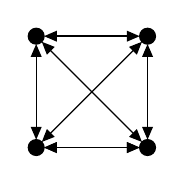
\begin{tikzpicture}[rotate=-45]
  \GraphInit[vstyle=Simple]
  \SetVertexSimple[MinSize=5pt]
  \renewcommand * {\EdgeLineWidth}{0.5pt}
  \Vertices{circle}{A,B,C,D}
  \Edges[style={{Triangle[angle=45:5pt]}-{Triangle[angle=45:5pt]}}](C,B,A,D,C,A,D,B)
\end{tikzpicture}

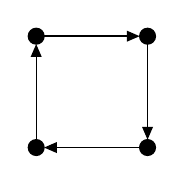
\begin{tikzpicture}[rotate=-45]
  \GraphInit[vstyle=Simple]
  \SetVertexSimple[MinSize=5pt]
  \renewcommand * {\EdgeLineWidth}{0.5pt}
  \Vertices{circle}{A,B,C,D}
  \Edges[style={-{Triangle[angle=45:5pt]}}](C,B,A,D,C)
\end{tikzpicture}

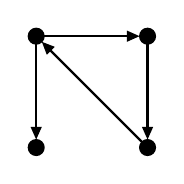
\begin{tikzpicture}[rotate=-45] 
  \GraphInit[vstyle=Simple]
  \SetVertexSimple[MinSize=5pt]
  \Vertices{circle}{A,B,C,D}
  \Edges[style={-{Triangle[angle=45:5pt]}}](C,B,A,C,D)
\end{tikzpicture}

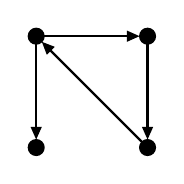
\begin{tikzpicture}[rotate=-45] 
  \GraphInit[vstyle=Simple]
  \SetVertexSimple[MinSize=5pt]
  \Vertices{circle}{A,B,C,D}
  \Edges[style={-{Triangle[angle=45:5pt]}}](C,B,A,C,D)
\end{tikzpicture}

%%%%%%%%%%%%%%%%%%%%%%%%%%%%%%%%%%%%%%%%%%%%%%%%%%%%%%%%%%%%%%%%%%%%%%%%%%%%%%%%%%%%%%%%%%%%%%%%%%%%%%

% {0,1} 

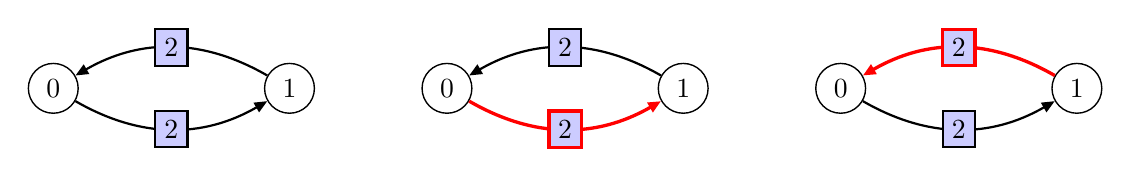
\begin{tikzpicture}
\SetGraphUnit{3}
\GraphInit[vstyle=Dijkstra]
\tikzset{EdgeStyle/.style = {-{Triangle[angle=45:5pt]},bend right,thick}}
\tikzset{LabelStyle/.style= {draw,fill = blue!20}}
\Vertex{0}
\EA(0){1}
\Edge[label=$2$](1)(0)
\Edge[label=$2$](0)(1)
\begin{scope}[xshift=5cm]
\SetGraphUnit{3}
\GraphInit[vstyle=Dijkstra]
\tikzset{EdgeStyle/.style = {-{Triangle[angle=45:5pt]},bend right,thick}}
\tikzset{LabelStyle/.style= {draw,fill=blue!20}}
\Vertex{0}
\EA(0){1}
\Edge[label=$2$](1)(0)
\SetUpEdge[style={draw=red,very thick,-{Triangle[angle=45:5pt]}, bend right}]
\tikzset{LabelStyle/.style ={draw,fill=blue!20}}
\Edge[label=$2$](0)(1)
\end{scope}
\begin{scope}[xshift=10cm]
\SetGraphUnit{3}
\GraphInit[vstyle=Dijkstra]
\tikzset{EdgeStyle/.style = {-{Triangle[angle=45:5pt]},bend right,thick}}
\tikzset{LabelStyle/.style= {draw,fill=blue!20}}
\Vertex{0}
\EA(0){1}
\Edge[label=$2$](0)(1)
\SetUpEdge[style={draw=red,very thick,-{Triangle[angle=45:5pt]}, bend right}]
\tikzset{LabelStyle/.style ={draw,fill=blue!20}}
\Edge[label=$2$](1)(0)
\end{scope}
\end{tikzpicture}


%VAN A EXISTIR 4 CASOS IMPORTANTES QUE DEBEMOS CONSIDERAR PARAFORMAR LAS PALABRAS CORTAS

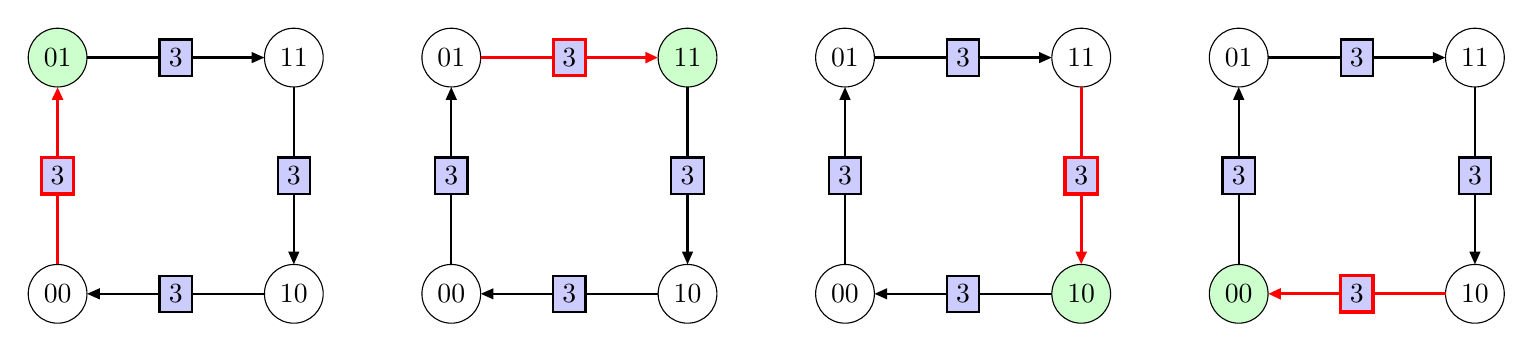
\begin{tikzpicture}
\SetGraphUnit{3}
\GraphInit[vstyle=Dijkstra]
\tikzset{LabelStyle/.style= {draw, fill = blue!20}}
\tikzset{VertexStyle/.style = {shape = circle, fill = green!20, draw}}
\Vertex {01}
\tikzset{VertexStyle/.style = {shape = circle, fill = white, draw}}
\EA(01){11} 
\SO(11){10}
\WE(10){00}
\Edges[style={-{Triangle[angle=45:5pt]}}, label=$3$](01,11)
\Edges[style={-{Triangle[angle=45:5pt]}}, label=$3$](11,10)
\Edges[style={-{Triangle[angle=45:5pt]}}, label=$3$](10,00)
\SetUpEdge[style={draw=red,very thick,-{Triangle[angle=45:5pt]}}]
\tikzset{LabelStyle/.style ={draw,fill=blue!20}}
\Edges[label=$3$](00,01)
\begin{scope}[xshift=5cm]
\SetGraphUnit{3}
\GraphInit[vstyle=Dijkstra]
\tikzset{LabelStyle/.style= {draw,
fill = blue!20}}
\Vertex {01}
\tikzset{VertexStyle/.style = {shape = circle, fill = green!20, draw}} 
\EA(01){11}
\tikzset{VertexStyle/.style = {shape = circle, fill = white, draw}}
\SO(11){10} 
\WE(10){00}
\Edges[style={-{Triangle[angle=45:5pt]}}, label=$3$](11,10)
\Edges[style={-{Triangle[angle=45:5pt]}}, label=$3$](10,00)
\Edges[style={-{Triangle[angle=45:5pt]}}, label=$3$](00,01)
\SetUpEdge[style={draw=red,very thick,-{Triangle[angle=45:5pt]}}]
\tikzset{LabelStyle/.style ={draw,fill=blue!20}}
\Edges[label=$3$](01,11)
\end{scope}
\begin{scope}[xshift=10cm]
\SetGraphUnit{3}
\GraphInit[vstyle=Dijkstra]
\tikzset{LabelStyle/.style= {draw,
fill = blue!20}}
\Vertex {01}
\EA(01){11} 
\tikzset{VertexStyle/.style = {shape = circle, fill = green!20, draw}} 
\SO(11){10}
\tikzset{VertexStyle/.style = {shape = circle, fill = white, draw}}
\WE(10){00}
\Edges[style={-{Triangle[angle=45:5pt]}}, label=$3$](10,00)
\Edges[style={-{Triangle[angle=45:5pt]}}, label=$3$](00,01)
\Edges[style={-{Triangle[angle=45:5pt]}}, label=$3$](01,11)
\SetUpEdge[style={draw=red,very thick,-{Triangle[angle=45:5pt]}}]
\tikzset{LabelStyle/.style ={draw,fill=blue!20}}
\Edges[label=$3$](11,10)
\end{scope}
\begin{scope}[xshift=15cm]
\SetGraphUnit{3}
\GraphInit[vstyle=Dijkstra]
\tikzset{LabelStyle/.style= {draw, fill = blue!20}}
\Vertex {01}
\EA(01){11}
\SO(11){10}
\tikzset{VertexStyle/.style = {shape = circle, fill = green!20, draw}} 
\WE(10){00}
\Edges[style={-{Triangle[angle=45:5pt]}}, label=$3$](00,01)
\Edges[style={-{Triangle[angle=45:5pt]}}, label=$3$](01,11)
\Edges[style={-{Triangle[angle=45:5pt]}}, label=$3$](11,10)
\SetUpEdge[style={draw=red,very thick,-{Triangle[angle=45:5pt]}}]
\tikzset{LabelStyle/.style ={draw,fill=blue!20}}
\Edges[label=$3$](10,00)
\end{scope}
\end{tikzpicture}

%%%%%%%%%%%%%%%%%%%%%%%%%%%%%%%%%%%%%%%%%%%%%%%%

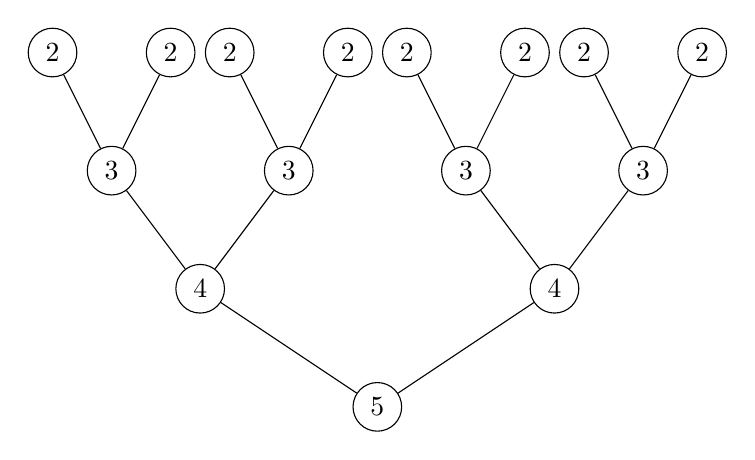
\begin{tikzpicture}[rotate=180,level/.style={sibling distance=45mm/#1}]
\tikzstyle{every node}=[draw,circle]
\node {5}
    child {node {4}
        child {node {3}
            child{node {2}}
            child{node {2}}
        }
        child {node {3}
            child{node {2}}
            child{node {2}}
        } 
    }
    child {node {4}
        child {node {3}
            child{node {2}}
            child{node {2}}
            }
        child {node {3}
            child{node {2}}
            child{node {2}}
            }
    };
\end{tikzpicture}



%%%%%%%%%%%%%%%%%%%%%%%%%%%%%%%%%%%%%%%%%%%%%%%%


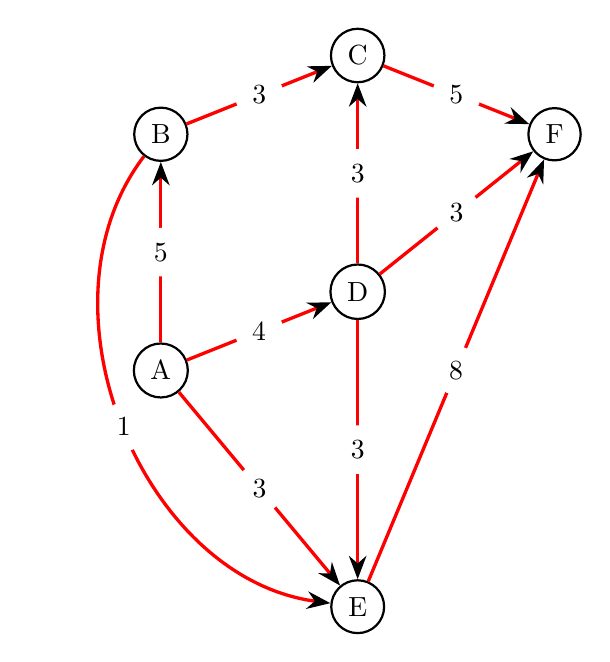
\begin{tikzpicture}
\begin{scope}[every node/.style={circle,thick,draw}]
    \node (A) at (0,0) {A};
    \node (B) at (0,3) {B};
    \node (C) at (2.5,4) {C};
    \node (D) at (2.5,1) {D};
    \node (E) at (2.5,-3) {E};
    \node (F) at (5,3) {F} ;
\end{scope}

\begin{scope}[>={Stealth[black]},
              every node/.style={fill=white,circle},
              every edge/.style={draw=red,very thick}]
    \path [->] (A) edge node {$5$} (B);
    \path [->] (B) edge node {$3$} (C);
    \path [->] (A) edge node {$4$} (D);
    \path [->] (D) edge node {$3$} (C);
    \path [->] (A) edge node {$3$} (E);
    \path [->] (D) edge node {$3$} (E);
    \path [->] (D) edge node {$3$} (F);
    \path [->] (C) edge node {$5$} (F);
    \path [->] (E) edge node {$8$} (F); 
    \path [->] (B) edge[bend right=60] node {$1$} (E); 
\end{scope}
\end{tikzpicture}

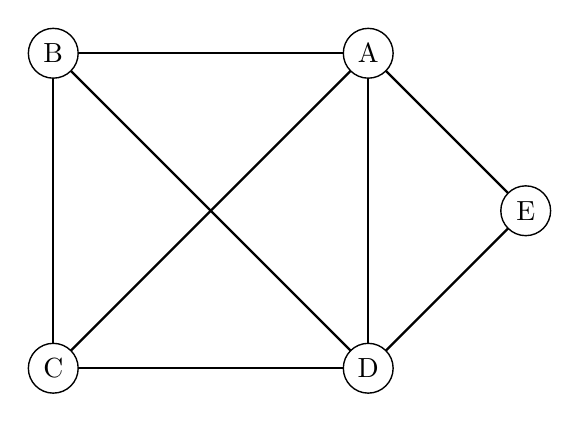
\begin{tikzpicture}
\SetGraphUnit{2}
\coordinate (O) at (0,0);
\NOEA(O){A} \NOWE(O){B} \SOEA(O){D}
\SOWE(O){C} \NOEA(D){E}
\Edges(B,C,D,A,E,D,B,A,C)
\end{tikzpicture}

  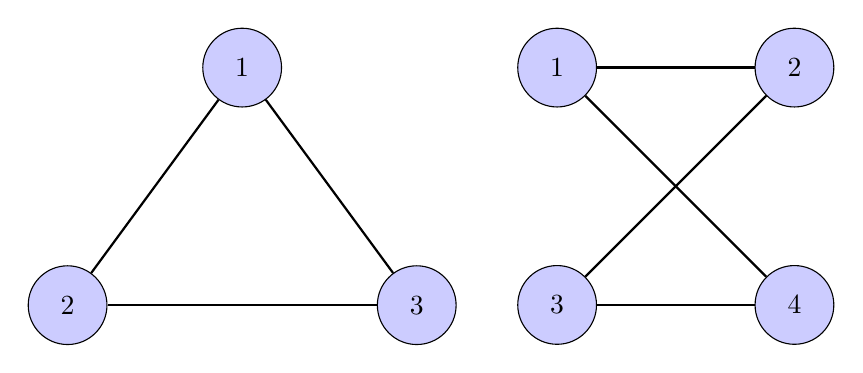
\begin{tikzpicture}
    \node[main node] (1) {$1$};
    \node[main node] (2) [below left = 2.3cm and 1.5cm of 1]  {$2$};
    \node[main node] (3) [below right = 2.3cm and 1.5cm of 1] {$3$};

    \path[draw,thick]
    (1) edge node {} (2)
    (2) edge node {} (3)
    (3) edge node {} (1);
    %%
    \begin{scope}[xshift=4cm]
    \node[main node] (1) {$1$};
    \node[main node] (2) [right = 2cm  of 1]  {$2$};
    \node[main node] (3) [below = 2cm  of 1] {$3$};
    \node[main node] (4) [right = 2cm  of 3] {$4$};

    \path[draw,thick]
    (1) edge node {} (2)
    (1) edge node {} (4)
    (3) edge node {} (2)
    (3) edge node {} (4)
    ;
    \end{scope}
\end{tikzpicture}


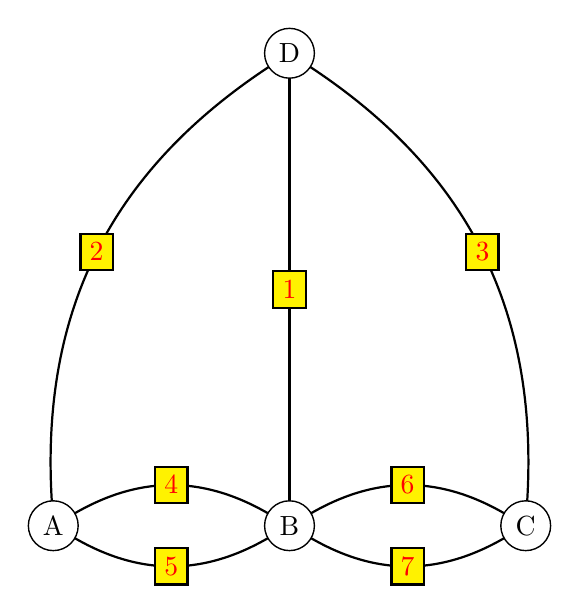
\begin{tikzpicture}
\SetGraphUnit{3}
\tikzset{LabelStyle/.style= {draw,
fill = yellow,
text = red}}
\Vertex{A}
\EA(A){B}
\EA(B){C}
\SetGraphUnit{6}
% modifie la distance entre les nodes
\NO(B){D}
\Edge[label=1](B)(D)
\tikzset{EdgeStyle/.append style = {bend left}}
\Edge[label=4](A)(B)
\Edge[label=5](B)(A)
\Edge[label=6](B)(C)
\Edge[label=7](C)(B)
\Edge[label=2](A)(D)
\Edge[label=3](D)(C)
\end{tikzpicture}

%%%%%%%%%%%%%%%%%%%%%%%%%%%%%%%%%%%%%%%%%%%%%%%%%

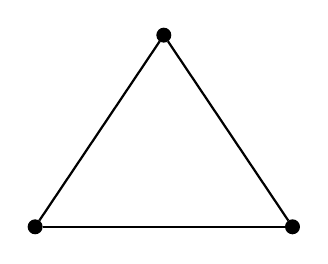
\begin{tikzpicture}
    \node[simple node] (1) {};
    \node[simple node] (2) [below left = 2.3cm and 1.5cm of 1]  {};
    \node[simple node] (3) [below right = 2.3cm and 1.5cm of 1] {};

    \path[draw,thick]
    (1) edge node {} (2)
    (2) edge node {} (3)
    (3) edge node {} (1);
    %%
\end{tikzpicture}
%\SetGraphUnit{4}

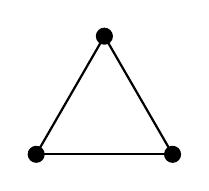
\begin{tikzpicture}[rotate=90]
\GraphInit[vstyle=Simple]
\SetVertexSimple[MinSize=5pt]
  \Vertices[NoLabel]{circle}{A,B,C}
  \Edges(A,B,C,A)
\end{tikzpicture}

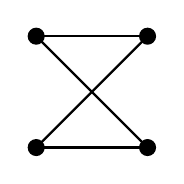
\begin{tikzpicture}[rotate=-45]
  \GraphInit[vstyle=Simple]
\SetVertexSimple[MinSize=5pt]
  \Vertices{circle}{A,B,C,D}
  \Edges(A,C,B,D,A)
\end{tikzpicture}
%%%%%%%%%%%%%%%%%%%%%%%%%%%%%%%%%%%%%%%%%%%%%%%%%%%

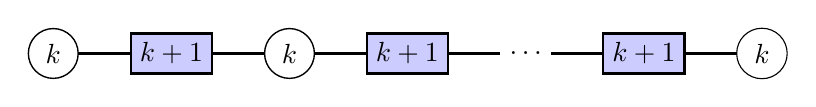
\begin{tikzpicture}
\SetGraphUnit{3}
\tikzset{LabelStyle/.style= {draw, fill = blue!20}}
\Vertex[L=$k$]{A}
\EA[L=$k$](A){B}
\tikzset{VertexStyle/.style = {draw=none,fill=none, text = black}}
\EA[L=$\ldots$](B){C}
\tikzset{VertexStyle/.style = {shape=circle, text = black, draw}}
\EA[L=$k$](C){D}
\Edge[label=$k+1$](A)(B)
\Edge[label=$k+1$](B)(C)
\Edge[label=$k+1$](C)(D)
\end{tikzpicture}

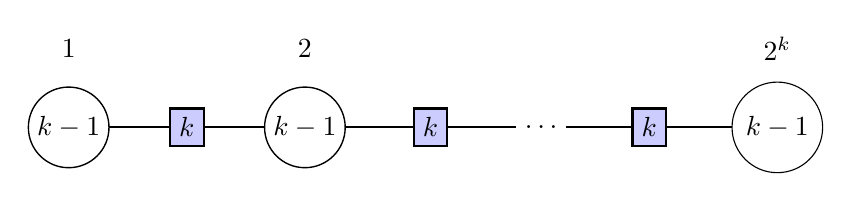
\begin{tikzpicture}
\SetGraphUnit{3}
\tikzset{LabelStyle/.style= {draw, fill = blue!20}}
\Vertex[L=$k-1$]{A}
\EA[L=$k-1$](A){B}
\tikzset{VertexStyle/.style = {draw=none,fill=none, text = black}}
\EA[L=$\ldots$](B){C}
\tikzset{VertexStyle/.style = {shape=circle, text = black, draw}}
\EA[L=$k-1$](C){D}
\Edge[label=$k$](A)(B)
\Edge[label=$k$](B)(C)
\Edge[label=$k$](C)(D)
\draw node [above of=A] {$1$};
\draw node [above of=B] {$2$};
\draw node [above of=D] {$2^k$};
\end{tikzpicture}

\end{document}